\documentclass[aoas]{imsart}
\setattribute{journal}{name}{}

\newcommand{\ba}{ {\boldsymbol a} }
\newcommand{\bA}{ {\boldsymbol A} }
\newcommand{\bb}{ {\boldsymbol b} }
\newcommand{\bB}{ {\boldsymbol B} }
\newcommand{\bc}{ {\boldsymbol c} }
\newcommand{\bC}{ {\boldsymbol C} }
\newcommand{\bd}{ {\boldsymbol d} }
\newcommand{\bD}{ {\boldsymbol D} }
\newcommand{\be}{ {\boldsymbol e} }
\newcommand{\bE}{ {\boldsymbol E} }
\newcommand{\boldf}{ {\boldsymbol f} }
\newcommand{\bF}{ {\boldsymbol F} }
\newcommand{\bg}{ {\boldsymbol g} }
\newcommand{\bG}{ {\boldsymbol G} }
\newcommand{\bh}{ {\boldsymbol h} }
\newcommand{\bH}{ {\boldsymbol H} }
\newcommand{\bi}{ {\boldsymbol i} }
\newcommand{\bI}{ {\boldsymbol I} }
\newcommand{\bj}{ {\boldsymbol j} }
\newcommand{\bJ}{ {\boldsymbol J} }
\newcommand{\bk}{ {\boldsymbol k} }
\newcommand{\bK}{ {\boldsymbol K} }
\newcommand{\bl}{ {\boldsymbol l} }
\newcommand{\bL}{ {\boldsymbol L} }
\newcommand{\bm}{ {\boldsymbol m} }
\newcommand{\bM}{ {\boldsymbol M} }
\newcommand{\bn}{ {\boldsymbol n} }
\newcommand{\bN}{ {\boldsymbol N} }
\newcommand{\bo}{ {\boldsymbol o} }
\newcommand{\bO}{ {\boldsymbol O} }
\newcommand{\bp}{ {\boldsymbol p} }
\newcommand{\bP}{ {\boldsymbol P} }
\newcommand{\bq}{ {\boldsymbol q} }
\newcommand{\bQ}{ {\boldsymbol Q} }
\newcommand{\br}{ {\boldsymbol r} }
\newcommand{\bR}{ {\boldsymbol R} }
\newcommand{\bs}{ {\boldsymbol s} }
\newcommand{\bS}{ {\boldsymbol S} }
\newcommand{\bt}{ {\boldsymbol t} }
\newcommand{\bT}{ {\boldsymbol T} }
\newcommand{\bu}{ {\boldsymbol u} }
\newcommand{\bU}{ {\boldsymbol U} }
\newcommand{\bv}{ {\boldsymbol v} }
\newcommand{\bV}{ {\boldsymbol V} }
\newcommand{\bw}{ {\boldsymbol w} }
\newcommand{\bW}{ {\boldsymbol W} }
\newcommand{\bx}{ {\boldsymbol x} }
\newcommand{\bX}{ {\boldsymbol X} }
\newcommand{\by}{ {\boldsymbol y} }
\newcommand{\bY}{ {\boldsymbol Y} }
\newcommand{\bz}{ {\boldsymbol z} }
\newcommand{\bZ}{ {\boldsymbol Z} }
\newcommand{\vc}[1]{\mbox{\boldmath $#1$}}
\newcommand{\balph}{ {\boldsymbol \alpha} }
\newcommand{\balpha}{ {\boldsymbol \alpha} }
\newcommand{\bbet}{ {\boldsymbol \beta} }
\newcommand{\bbeta}{ {\boldsymbol \beta} }
\newcommand{\bgam}{ {\boldsymbol \gamma} }
\newcommand{\bgamma}{ {\boldsymbol \gamma} }
\newcommand{\bGamma}{ {\boldsymbol \Gamma} }
\newcommand{\bdelta}{ {\boldsymbol \delta} }
\newcommand{\bDelta}{ {\boldsymbol \Delta} }
\newcommand{\beps}{ {\boldsymbol \epsilon} }
\newcommand{\bepsilon}{ {\boldsymbol \epsilon} }
\newcommand{\bphi}{ {\boldsymbol \phi} }
\newcommand{\bPhi}{ {\boldsymbol \Phi} }
\newcommand{\bpi}{ {\boldsymbol \pi} }
\newcommand{\bpsi}{ {\boldsymbol \psi} }
\newcommand{\bkap}{ {\boldsymbol \kappa} }
\newcommand{\bkappa}{ {\boldsymbol \kappa} }
\newcommand{\bKappa}{ {\boldsymbol \Kappa} }
\newcommand{\blam}{ {\boldsymbol \lambda} }
\newcommand{\blambda}{ {\boldsymbol \lambda} }
\newcommand{\bLambda}{ {\boldsymbol \Lambda} }
\newcommand{\bmu}{ {\boldsymbol \mu} }
\newcommand{\bMu}{ {\boldsymbol \Mu} }
\newcommand{\bet}{ {\boldsymbol \eta} }
\newcommand{\bome}{ {\boldsymbol \omega} }
\newcommand{\bomega}{ {\boldsymbol \omega} }
\newcommand{\bOmega}{ {\boldsymbol \Omega} }
\newcommand{\bnabla}{ {\boldsymbol \nabla} }
\newcommand{\brho}{ {\boldsymbol \rho} }
\newcommand{\bsigma}{ {\boldsymbol \sigma} }
\newcommand{\bSig}{ {\boldsymbol \Sigma} }
\newcommand{\bSigma}{ {\boldsymbol \Sigma} }
\newcommand{\btheta}{ {\boldsymbol \theta} }
\newcommand{\bTheta}{ {\boldsymbol \Theta} }
\newcommand{\bzeta}{ {\boldsymbol \zeta} }
\newcommand{\bPsi}{ {\boldsymbol \Psi} }
\newcommand{\btau}{ {\boldsymbol \tau} }
\newcommand{\bxi}{ {\boldsymbol \xi} }
\newcommand{\bzero}{ {\boldsymbol 0} }
\newcommand{\bones}{ {\boldsymbol 1} }
\newcommand{\given}{\,|\,}
\newcommand{\sS}{{\cal S}}
\newcommand{\Ss}{{\cal S}}
\newcommand{\Field}{{\cal F}}
\newcommand{\colsp}{{\cal C}}
\newcommand{\nullsp}{{\cal N}}
\newcommand{\rowsp}{{\cal R}}
\newcommand{\tildeC}{\tilde{C}}
\newcommand{\tildeK}{\tilde{K}}
\newcommand{\tildew}{\tilde{w}}
\newcommand{\tildebw}{\tilde{\bw}}
\newcommand{\tildebW}{\tilde{\bW}}
\newcommand{\calC}{{\cal C}}
\newcommand{\calcbC}{{\bf {\cal C}}}

% Do not remove even for final version
\newcommand{\kcomment}[1]{{\color{blue}{\{KR: #1\}}}}
\newcommand{\kc}{\kcomment}


\usepackage{amsmath}
\usepackage{pstricks,pst-grad}
\usepackage{graphicx}
\usepackage{floatrow}
\usepackage[linesnumbered,ruled,vlined]{algorithm2e}
\floatsetup[table]{capposition=top}
\usepackage{subfigure}
\usepackage[utf8]{inputenc}
\usepackage{booktabs}                     % horizontal lines in tables
\usepackage{comment}

\usepackage{textcomp}
\usepackage{amsthm,amsmath,natbib}
%\RequirePackage[colorlinks,citecolor=blue,urlcolor=blue]{hyperref}
\usepackage{color, colortbl}
\definecolor{Gray}{gray}{0.9}

\usepackage{amssymb}
\usepackage{hyperref}
\usepackage{cleveref}
\usepackage{xcolor}
% For testing whether an argument of a macro is empty.
\usepackage{xifthen}
\usepackage{bm}
\usepackage{bbm}

\newcommand{\dl}{\mathrm{d}\lambda}
\newcommand{\R}{\mathbb{R}}
\newcommand{\x}{s}
\newcommand{\uu}{u}
\newcommand{\vv}{v}
%\newcommand{\bt}{t}
\newcommand{\T}{T}
\newcommand{\es}{\Gamma}%\mathrm{ES}}
\newcommand{\ibv}{\mathrm{IBV}}
\newcommand{\emv}{\mathrm{EMV}}
\newcommand{\eibv}{\mathrm{EIBV}}
\newcommand{\eemv}{\mathrm{EEMV}}
\newcommand{\mes}{\nu}
% \newcommand{\gp}{\xi}
\newcommand{\no}{p}
\newcommand{\eps}{\varepsilon}
\newcommand{\sigeps}{\Sigma_{\eps}}
\newcommand{\cov}{\operatorname{Cov}}
\newcommand{\norm}{\mathcal{N}}
\newtheorem{propo}{Proposition}
\newtheorem{theorem}{Theorem}
\newtheorem{remark}{Remark}
\newtheorem*{remark*}{Remark}


\DeclareMathOperator*{\argmin}{\arg\!\min}

% Mean and cov at time zero.
\newcommand{\mean}[1]{\mu
\left(#1\right)}
\newcommand{\covmat}[1]{K
\left(#1\right)}

% Product measure.
\newcommand{\productMeasure}{
\mathrm{d}\nu^{\otimes}\left(\bm{u}\right)}

% Field value at x. Can either switch between parenthesis or subscripting.
% If no argument provided, then will just print xi.
\newcommand{\gp}[1][]{
    \ifthenelse{\isempty{#1}}
    {Z}
    {Z_{#1}}
}

% Misc. covariance matrices
\newcommand{\covV}{C_{V}}
\newcommand{\covN}{C}


% Covariance function k(., .).
\newcommand{\covFunc}[4]{k_{#2#4}\left(#1,#3\right)}

% Covariance matrix K = k(X, X).
\newcommand{\covMat}[4]{\bm{K}_{#2#4}(#1#3)}

% Mean function \mu(x).
\newcommand{\meanFunc}[2]{\mu_{#2}\left(#1\right)}

% Mean vector \mu(X).
\newcommand{\meanVec}[2]{\bm{\mu}_{#2}(#1)}

% Excursion probability in the set T^r.
\newcommand{\jointExcuProb}{
    \mathbb{P}\left(
    \gp[\bm{u}]\in T^r \right)
}

% In Proposition 1, the mean vector at the uu concatenation and the
% corresponding covariance matrix.
\newcommand{\meanUU}{
    \mu(\bm{u})
}

\newcommand{\covUU}{
    K\left(\bm{u},\bm{u}\right)
}

% ----------
% SEQUENTIAL
% ----------
% Probability distribution now (after 1 conditioning).
\newcommand{\currentProba}[1]{\mathbb{P}_{[n]}
\left(#1\right)}
% Probability distribution in the future (after 2 conditioning).
\newcommand{\futureProba}[1]{\mathbb{P}_{[n+1]}
\left(#1\right)}

% Same for expectations.
\newcommand{\currentExp}[1]{\mathbb{E}_{[n]}
\left[#1\right]}
\newcommand{\futureExp}[1]{\mathbb{E}_{[n+1]}
\left[#1\right]}

% For mean vectors.
\newcommand{\currentMean}[1]{\mu_{[n]}
\left(#1\right)}
\newcommand{\futureMean}[1]{\mu_{[n+1]}
\left(#1\right)}

% And covariance matrices.
\newcommand{\currentCov}[1]{K_{[n]}
\left(#1\right)}
\newcommand{\futureCov}[1]{K_{[n+1]}
\left(#1\right)}


% For nice expectations.
\usepackage{mathtools}
\newcommand{\expect}{\mathbb{E}\expectarg}
\DeclarePairedDelimiterX{\expectarg}[1]{[}{]}{%
  \ifnum\currentgrouptype=16 \else\begingroup\fi
  \activatebar#1
  \ifnum\currentgrouptype=16 \else\endgroup\fi
}

\newcommand{\innermid}{\nonscript\;\delimsize\vert\nonscript\;}
\newcommand{\activatebar}{%
  \begingroup\lccode`\~=`\|
  \lowercase{\endgroup\let~}\innermid
  \mathcode`|=\string"8000
}


\begin{document}

\begin{frontmatter}

\title{Supplementary Materials for Learning Excursion Sets of Vector-valued Gaussian Random Fields for
Autonomous Ocean Sampling}


\begin{aug}
\author{\fnms{Trygve Olav} \snm{Fossum}\thanksref{t1,t2}, \corref{} \ead[label=e1]{trygve.o.fossum@ntnu.no}}
\author{\fnms{Cédric} \snm{Travelletti}\thanksref{t3}, \corref{} \ead[label=e2]{cedric.travelletti@stat.unibe.ch}}
\author{\fnms{Jo} \snm{Eidsvik}\thanksref{t4}, \ead[label=e3]{jo.eidsvik@ntnu.no}}
\author{\fnms{David} \snm{Ginsbourger}\thanksref{t3}, \ead[label=e4]{david.ginsbourger@stat.unibe.ch}}
\and
\author{\fnms{Kanna} \snm{Rajan}\thanksref{t5,t6}. \ead[label=e5]{kanna.rajan@fe.up.pt}}

\affiliation[t1]{Department of Marine Technology, The Norwegian University of Science and Technology (NTNU), Trondheim, Norway.} 
\affiliation[t2]{Centre for Autonomous Marine Operations and Systems, NTNU.}
\affiliation[t3]{Institute of Mathematical Statistics and Actuarial Science, University of Bern, Switzerland.}
\affiliation[t4]{Department of Mathematical Sciences, NTNU.}
\affiliation[t5]{Underwater Systems and Technology Laboratory, Faculty of Engineering, University of Porto, Portugal.}
\affiliation[t6]{SIFT LLC, Minneapolis, Minnesota, United States.}

\address{Trygve Olav Fossum \\Department of Marine Technology\\ Otto Nielsens veg. 10, 7491 Trondheim\\ Norway\\
\printead{e1}}
\address{Cédric Travelletti\\ Institute of Mathematical Statistics and Actuarial Science \\ University of Bern \\
Switzerland.
\printead{e2}}
\address{Jo Eidsvik\\Department of Mathematical Sciences\\ Hogskoleringen 1, 7491 Trondheim\\ Norway\\ \printead{e3}}
\address{David Ginsbourger\\ Institute of Mathematical Statistics and Actuarial Science \\ University of Bern \\
Switzerland.
\printead{e4}}
\address{Kanna Rajan\\Underwater Systems and Technology Laboratory,
  Faculty of Engineering,\\ Rua Dr. Roberto Frias\\ University of Porto, Portugal\\
\printead{e5}}

\runauthor{TO. Fossum et al.}
\end{aug}
\end{frontmatter}

\textbf{The PDF file includes:} Supplementary materials to the manuscript ``Learning Excursion Sets of Vector-valued Gaussian Random Fields for
Autonomous Ocean Sampling" by Fossum et. al 2021. 

\section{Derivation of proofs}
\setcounter{propo}{2}
\begin{propo}
    \label{propo1}
%Under technical conditions to be precised, $\mu(\es)$ possesses moments or arbitrary order and these can be expressed for any $r\geq 1$ as
For a measurable random field $\gp$ and a locally finite measure $\mes$ on $\domain$, $\mes(\es)$ is a random variable and for 
any $r\geq 1$,
\begin{equation*}
\begin{split}
\mathbb{E}[\mes(\es)^r]
&=\int_{\domain^{r}} \jointExcuProb
\productMeasure
,
\end{split}
\end{equation*}

where the product measure is denoted as
$\nu^{\otimes}:=\bigotimes_{i=1}^r \nu$.
%Note that we will use boldface to denote concatenated variables. % TO RELOCATE
Here $\gp$ is defined on $\domain$, and for
$\bm{u}=\left(u^{(1)}, ..., u^{(r)}\right)\in \domain^r$, $\gp[\bm{u}]=\left(\gp[u^{(1)}], ...,
\gp[u^{(r)}]\right)\in \mathbb{R}^{\no r}$.
\medskip

In the particular case where $\gp$ is a multivariate Gaussian random field
%and denoting the mean and covariance matrix of $\gp[\bm{u}]$ by $\meanUU\in\mathbb{R}^{p\times r}$ and $\covUU$, respectively,
we have
\begin{align*}
\jointExcuProb = \mathcal{N}_{\no r}(T^r; \meanUU, \covUU),
\end{align*}
where $\mathcal{N}_{\no r}(\cdot ; \meanUU, \covUU)$ is the Gaussian measure on $\mathbb{R}^{\no r}$ with mean $\meanUU$ 
and covariance matrix $\covUU$, respectively defined blockwise by
%where both are defined blockwise by
\begin{align*}
\meanUU&=\begin{pmatrix}\mu(u^{(1)})\\ \vdots\\ \mu(u^{(r)})\end{pmatrix}
\in \mathbb{R}^{\no r}, \\
\text{and } \covUU &= \begin{pmatrix}
\cov(\gp[u^{(1)}], \gp[u^{(1)}]) & \dots & \cov(\gp[u^{(1)}],
\gp[u^{(r)}])\\
\vdots & & \vdots\\
\cov(\gp[u^{(r)}], \gp[u^{(1)}]) & \dots & \cov(\gp[u^{(r)}],
\gp[u^{(r)}])\\
\end{pmatrix}\in \mathbb{R}^{pr\times pr},
\end{align*}
each of the $r\times r$ blocks of the latter matrix being itself a (cross-)covariance matrix of dimension $\no \times 
\no$.
%dimensional Gaussian random vector.
Assuming further that $\covUU$ is non-singular, the probability of interest can be formulated in terms of the $\no 
r$-dimensional Gaussian probability density function
$\varphi_{\no  r}(\cdot;~\meanUU, \covUU)$ as
%$\varphi_{\no \times r}$ as
%$\bm{u}\in D^r$ such that $\gp[\bm{u}]$ be non-degenerate, the integrand can be expressed in terms of the $r \times \no$-dimensional Gaussian distribution, namely
%cumulative distribution function, namely
\begin{equation*}
\begin{split}
&\jointExcuProb
=
\int_{T^r} \varphi_{\no  r}\left(\bm{v};
    ~\meanUU, \covUU\right)
    \mathrm{d}\bm{v},
\end{split}
\end{equation*}
In the particular orthant case with $\T=(-\infty, t_1] \times \dots \times (-\infty, t_{r}]$,
the latter probability directly writes in terms of the multivariate Gaussian
cumulative distribution, % with mean $\meanUU$ and covariance matrix $\covUU$,
this time by the way without requiring $\covUU$ %the latter
to be non-singular:
\begin{equation*}
\begin{split}
\jointExcuProb
&=
\varPhi_{\no r}\left(\bm{t};~\meanUU, \covUU\right),
\end{split}
\end{equation*}
where we have used the notations
$t=(t_1,\dots,t_{\no}%,..., t_1, ..., t_p
)\in\mathbb{R}^{\no}$, $1_{r}=(1,\dots,1)\in \R^{r}$, and
$\bm{t}=1_{r}\otimes \bm{t}=(t_1,\dots,t_{\no},\dots,t_1,\dots,t_{\no})
\in \R^{\no r}$.
\end{propo}
\begin{proof}
That $\mes(\es)$ defines indeed a random variable follows from Fubini's theorem
relying on the joint measurability of
$(\x, \omega) \to \mathbbm{1}_{\es(\omega)}(\x)$,
%= \mathbf{1}_{\xi_{\x}(\omega) \in T}$ and Fubini's theorem.
itself inherited from the assumed measurability for
$(\x, \omega) \to \gp[\x](\omega)$ and $T$, respectively. From there, following the steps of Robbins' theorem \cite{Robbins1944}, we find that
\begin{equation*}
\begin{split}
\mathbb{E}[\mes(\es)^{r}]
&=\mathbb{E}\left[\left(\int_{\domain} \mathbbm{1}_{\gp[u] \in T} ~d\mes(u) \right)^{r} \right]
=\mathbb{E}\left[ \prod_{i=1}^{r} \left(
        \int_{\domain} \mathbbm{1}_{\gp[\uu^{(i)}] \in T} ~d\mes(\uu^{(i)})
\right) \right] \\
&
=
%\mathbb{E}\left[
%\int_{D^{r}}
%\prod_{i=1}^{r}
%\mathbf{1}_{\gp[\uu^{(i)}] \in T}
%\productMeasure
%\right]
%=
\mathbb{E}\left[
\int_{\domain^{r}}
\mathbbm{1}_{\gp[\uu^{(1)}] \in T,\dots, \gp[\uu^{(r)}]  \in T}
\productMeasure
\right]
%\\
%&=\int_{D^{r}} \mathbb{E}\left[\mathbf{1}_{\gp[\bm{u}] \in T^r} \right] \productMeasure \\
%&
=\int_{\domain^{r}}
\jointExcuProb
\productMeasure.
\end{split}
\end{equation*}
The rest consists in expliciting the probability of $T\times \dots \times T$ under the multivariate Gaussian distribution of
$\left(\gp[u^{(1)}], \dots,  \gp[u^{(r)}] \right)$.
\end{proof}

The propositions below provide formulae for computations of expectations of moments of multivariate gaussian CDFs.

\begin{propo}
    \label{propo2}
Let $p, q, h \geq 1$, $a \in \R^p$, $B \in \R^{p\times q}$,
and $\covN$, $\covV$ be two covariance matrices in
$\R^{p\times p}$ and $\R^{q\times q}$, respectively.
Then, for $V \sim \mathcal{N}_{q}(0_q, \covV)$,
\begin{equation*}
\mathbb{E}\left[ \varPhi_{p}\left( a + BV; \covN \right)^h \right]
=
\varPhi_{ph}
\left(
    \bm{a}
;~
\bm{\Sigma}
\right),
\end{equation*}
where the vector $\bm{a} \in \R^{p h}$ is defined as
$\bm{a} := 1_h\otimes a = 
\left(a, \dots , a
\right)'$
 and the $p h\times p h$ covariance matrix is given by
 $\bm{\Sigma} := 
1_h 1_h'\otimes B\covV B' + I_h\otimes \covN$.
\end{propo}

\begin{remark}
In blockwise representation, $\bm{\Sigma}$ can be expressed as follows:
\begin{align*}
% \bm{\Sigma}&=
\begin{pmatrix}
    \covN & &\\
        & \ddots &\\
        &   & \covN
\end{pmatrix}
+
\begin{pmatrix}
B\covV B' & \dots & B\covV  B'\\
\vdots & & \vdots\\
B\covV B' & \dots & B\covV B'\\
\end{pmatrix}
\end{align*}
\end{remark}

\begin{proof}
By definition of $\Phi_{p}$, for $N\sim \mathcal{N}_{p}(0_{p},\covN)$,
$$
\mathbb{P}(N\leq a + BV | V)
=
\varPhi_{p}\left( a + BV; \covN \right).
$$
Now for $\varPhi_{p}\left( a + BV; \covN \right)^h$, provided that the probability space is sufficiently large to accomodate $h$ independent Gaussian random vectors $N_i\sim \mathcal{N}_{p}(0,\covN)$ (which is silently assumed here), using the former equality delivers
$$
\varPhi_{p}\left( a + BV; \covN \right)^h
=
\prod_{i=1}^h \mathbb{P}(N_i\leq a + BV | V).
$$
Now by independence of the $N_i$'s we obtain the joint conditional probability
$$
\prod_{i=1}^h \mathbb{P}(N_i\leq a + BV | V)
=
\mathbb{P}(N_1\leq a + BV, \dots, N_h\leq a + BV| V),
$$
whereof, by virtue of the law of total expectation,
\begin{equation*}
\begin{split}
\mathbb{E}\left[ \varPhi_{p}\left( a + BV; \covN \right)^h \right]
&=\mathbb{E}\left[\mathbb{P}(N_1\leq a + BV, \dots, N_h\leq a + BV| V)\right]\\
&=\mathbb{P}(N_1\leq a + BV, \dots, N_h\leq a + BV)\\
&=\mathbb{P}(W_1 \leq a, \dots, W_h\leq a)\\
&=\varPhi_{ph}
\left(
1_{h} \otimes a
;
(1_{h}1_{h}')\otimes (B\Sigma_{V} B') + 
I_{h}\otimes \covN
\right),
\end{split}
\end{equation*}
where $\mathbf{W}=(W_1,\dots,W_h)$ with $W_i=N_i- BV \ (1\leq i \leq h)$
and the last line follows $\mathbf{W}$ forming a Gaussian vector (by global independence of the $N_i$'s and $V$) and from the definition of $\varPhi_{p h}$. The covariance matrix $\mathbf{\Sigma}$ of $\mathbf{W}$ is obtained by noting that $\operatorname{cov}(W_i,W_j)=B \covV B' + \delta_{ij} \covN \ 
(i,j \in \{1,\dots,h\})$.
%the latter concatenated Gaussian vector is obtained by straightfoward calculation. 
\end{proof}

We now generalize Proposition~\ref{propo2} to the case of multivariate monomials in orthant probabilities with thresholds affine in a common Gaussian vector.
%Namely, for monomials of degree $k$, we have.

\begin{propo}
    \label{propo3}
Let $g, p, q\geq 1$, $h_{1},\dots, h_{g}\geq 1$ with $H=\sum_{i=1}^g h_i$, $a_{i} \in \R^{p}$, $B_{i}\in \R^{p \times q}$, and covariance matrices $\covN_i \in \R^{p \times p}$ $(1\leq i \leq g)$. Then, for any covariance matrix $\covV \in \R^{q\times q}$ and $V\sim\mathcal{N}_{q}(0_q,\covV)$,
    \begin{equation}
    \mathbb{E}\left[ \prod_{i=1}^{g} \varPhi_{p}\left(a_i + B_{i}V; \covN_{i} \right)^{h_i} \right]
    =
\varPhi_{p H}
\left(
    \bm{a}
;
\mathbf{\Sigma}
\right),
\end{equation}
with $\bm{a}=(1_{h_1}\otimes a_1, \dots, 1_{h_g}\otimes a_{g}) \in \R^{p H}$
and $\mathbf{\Sigma}\in \R^{p H \times p H}$ is defined blockwise by $(\Sigma_{i,j})_{i,j \in \{1,\dots, g\}}$ where, for any $i,j \in \{1,\dots, g\}$, %the blocks are given by 
\begin{equation}
\Sigma_{i,j}=
(1_{h_{i}}1_{h_{j}}')\otimes (B_{i}\Sigma_{V} B_{j}') + \delta_{i,j}(I_{h_{i}}\otimes \covN_{i}) \in \R^{p h_{i} \times p h_{j}}.
\end{equation}
\end{propo}

\begin{remark}
Using blockwise representation for the blocks themselves delivers %$\bm{\Sigma}$ can be expressed as follows
\begin{equation*}
%    \bm{\Sigma} = \begin{pmatrix}
%        \Sigma_{11} & & \Sigma_{1g}\\
%        & \ddots &\\
%        \Sigma_{g1}&   & \Sigma_{gg}
%\end{pmatrix},~
\Sigma_{ij} =
\begin{pmatrix}
B_i\Sigma_{V} B_j' & \dots & B_i\Sigma_{V} B_j'\\
\vdots & & \vdots\\
B_i\Sigma_{V} B_j' & \dots & B_i\Sigma_{V} B_j'\\
\end{pmatrix}
+
\delta_{ij}
\begin{pmatrix}
    \covN_i & &\\
        & \ddots &\\
        &   & \covN_i
\end{pmatrix}%\in\mathbb{R}^{lh_i\times lh_j}
\end{equation*}
Here each $\Sigma_{ij}$ is made of $h_i$ times $h_j$
(vertically/horizontally) $p \times p$ sub-blocks, hence possesses $ph_i$ lines and $ph_j$ columns.
\end{remark}

\begin{proof}
    The proof relies (again) heavily on the fact that, by definition of $\Phi_{p}$, for any covariance matrix $\covN \in \R^{p \times p}$, $a\in \R^p$, $B\in \R^{p \times q}$, and $N\sim \mathcal{N}_{p}(0_{p},\covN)$,
    $$
    \mathbb{P}(N\leq a + BV | V)
    =
    \varPhi_{p}\left( a + BV; \covN \right).
    $$
In particular, for globally independent $N_{i,j} \sim \mathcal{N}_{p}(0_{p},\covN_i)$ $(1\leq j \leq h_i, 1\leq i \leq g)$,
\begin{equation*}
\begin{split}
\prod_{i=1}^{g} \varPhi_{p}\left(a_i + B_{i}V; \covN_{i} \right)^{h_i}
&=
\prod_{i=1}^{g}
\prod_{j=1}^{h_{i}}
\mathbb{P}(N_{i,j}\leq a_i + B_i V | V)\\
&=\mathbb{P}(N_{1,1}\leq a_1 + B_1 V, \dots, N_{g,h_{g}}\leq a_g + B_g V | V),
\end{split} 
\end{equation*}
so that, by the law of total expectation,
    \begin{equation*}
    \begin{split}
    \mathbb{E}\left[ \prod_{i=1}^{g} \varPhi_{p}\left(a_i + B_{i}V; \covN_{i} \right)^{h_i} \right]
=
\mathbb{P}(W_{1} \leq 1_{h_{1}} \otimes a_1, \dots, W_{g} \leq 1_{h_{g}} \otimes a_g)
    \end{split}
    \end{equation*}
where
$W_{1}=(N_{1,1}- B_1 V, \dots, N_{1,h_{1}}- B_1 V), 
W_{2}=(N_{2,1}- B_2 V, \dots, N_{2,h_{2}}- B_2 V), 
\dots, W_{g}=(N_{g,1}- B_g V, \dots, N_{g,h_{g}}- B_g V)$. Noting that $\mathbf{W}=(W_1,\dots, W_g)$ is a centred $p H$-dimensional Gaussian random vector, we finally obtain that
    \begin{equation*}
\begin{split}
\mathbb{E}\left[ \prod_{i=1}^{g} \varPhi_{p}\left(a_i + B_{i}V; \covN_{i} \right)^{h_i} \right]
=
\varPhi_{p H}\left(\bm{a};\mathbf{\Sigma}\right),
    \end{split}
\end{equation*}
with $\bm{a}=(1_{h_{1}} \otimes a_1, \dots, 1_{h_{g}} \otimes a_g)$ and $\bm{\Sigma}=(\operatorname{cov}(W_i,W_j))_{i,j \in \{1,\dots, g\}}$.
\end{proof}

Those two general results allow us to derive simple expressions for the expected effect of the inclusion of new datapoints on the $\IBV$ (Proposition 1) and on the $\EMV$ (Proposition 2) for which we provide proofs below.


\begin{proof}{(Proposition 1)}
Applying Tonelli-Fubini followed by the law of total
expectation first delivers
\begin{equation*}
\begin{split}
\eibv_{[n]}(\bm{x})
&=\int_{\domain}
\currentExp{\futureProba{\gp[\uu]\in
        T}(1-\futureProba{\gp[\uu]\in T})} d\mes(u) \\
&=\int_{\domain} \varPhi_{\no}\left(\bt;
~\futureMean{\uu},
\futureCov{u,u}\right) d\mes(u)\\
&-\int_{\domain} \currentExp{
    \varPhi_{\no}\left(\bt;
    ~\futureMean{\uu},
    \futureCov{u,u}\right)^2
}
d\mes(u), 
\end{split}
\end{equation*}
%
where $\futureCov{u,u}$ denotes the $\no \times \no$ covariance matrix between all $\no$
responses at point $u$ conditional on the first $n+1$ observation batches.
Now, by using co-kriging update formulae and our shortcut notation for the CDF of centred
multivariate Gaussian vectors, we observe that
\begin{equation*}
\begin{split}
%\mathbb{E}_{n}[\left(
&\varPhi_{\no}\left(\bt;~\futureMean{\uu}, \futureCov{u, u}\right) 
%\right)^2]
\\
=&
\varPhi_{\no}\left(\bt-\futureMean{\uu}; \futureCov{u, u}\right) \\
=&
\varPhi_{\no}\left(\bt-\currentMean{\uu}-\lambda_{[n+1,n+1]}(u)^T(\gp[\bm{x}_{n+1}]
-\currentMean{\bm{x}_{n+1}}), \futureCov{u, u}\right) \\
=&
\varPhi_{\no}\left(a + BV, \futureCov{u, u}\right),
\end{split}
\end{equation*}
with $a=\bt-\currentMean{\uu}$, %+\lambda_{[n+1,n+1]}(u)^T\currentMean{\bm{x}_{n+1}}$,
$B=-\lambda_{[n+1,n+1]}(u)^T$
and $V=\gp[\bm{x}_{n+1}]-\currentMean{\bm{x}_{n+1}}$.
Applying Proposition~\ref{propo2} then delivers that
%
\begin{equation*}
\begin{split}
&\currentExp{
    \varPhi_{\no}\left(\bt;~\futureMean{\uu}, \futureCov{u, u}\right)^2 
}
%\\
=\varPhi_{2\no}
\left(
\left(
\begin{matrix}
\bt-\currentMean{\uu}\\
%\vdots \\ 
%\vdots \\ 
%\vdots \\ 
\bt-\currentMean{\uu}
\end{matrix}
\right);
\mathbf{\Sigma}_{[\stage]}(\uu)
\right),
\end{split}
\end{equation*}
with $\mathbf{\Sigma}_{[n]}(\uu)$ as in the formulation of the proposition. This completes the proof.
\end{proof}


\begin{proof}{(Proposition 2)}
\begin{equation*}
\begin{split}
\currentEEMV(\bm{x})
%\operatorname{Var}[\mes(\es)]
&=\int_{\domain^2} 
\varPhi_{2\no}
\left(
(\bt, \bt); \mu((u,v)), 
K((u,v),(u,v))
\right) 
\
\mathrm{d}\mes^{\otimes} %\mes 
%\productMeasure 
(u,v)\\
&-\int_{\domain^2} 
\currentExp{
\varPhi_{\no}\left(\bt; \futureMean{\uu}, K_{[n+1]}(\uu, \uu)\right)
\varPhi_{\no}\left(\bt; \futureMean{\vv}, K_{[n+1]}(\vv, \vv)\right)
}
\
\mathrm{d}\mes^{\otimes} %\mes 
%\productMeasure 
(u,v)
\end{split}
\end{equation*}
and the proof follows by applying Proposition \ref{propo3}
with
$$V=\gp[\bm{x}_{n+1}]-\currentMean{\bm{x}_{n+1}} \sim \mathcal{N}(0_{q_{n+1}},k_{[n]}(\bm{x}_{n+1},\bm{x}_{n+1}))$$
and $a_1=\bt-\currentMean{\uu}$,
$B_1=-\lambda_{[n+1,n+1]}(\uu)^T$, $a_2=\bt-\currentMean{\vv}$, $B_2=-\lambda_{[n+1,n+1]}(\vv)^T$, $C_1 = \currentCov{\uu, \uu}$, $C_2 = \currentCov{\vv, \vv}$.
\end{proof}

\section{Discussion on nugget sensitivity}

In the field experiments, the initial survey transect had no samples at very short distance, and these data are hence not reliable for extracting the nugget effect. The sensor-provided standard deviations of the measurement tools are in the fourth decimal points, but based on our experience \citep{fossuminformation}, there is more variability than this in temperature and salinity measurements in water samples close in space and time. This variability is partly due to dynamic water masses but also uncertainty in the AUV position. 
\begin{figure}[h] 
\centering
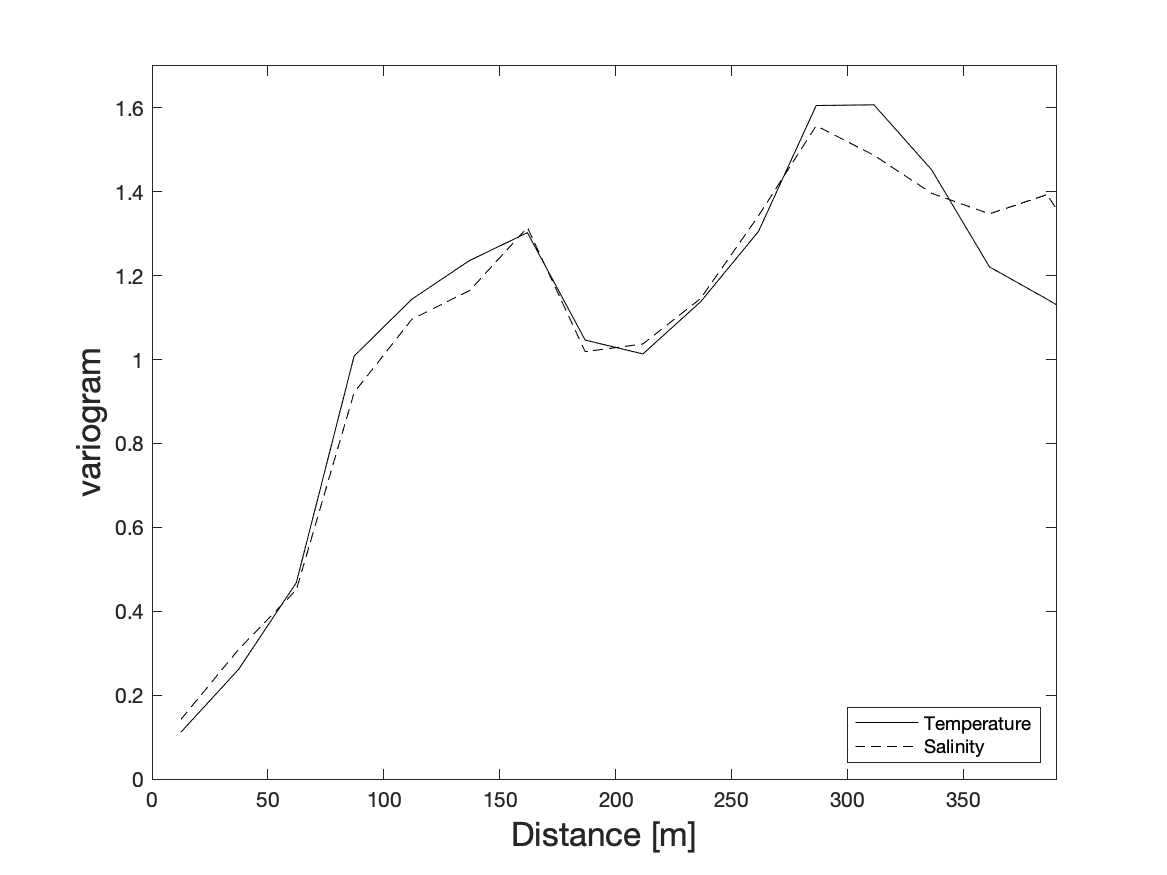
\includegraphics[width=0.6\textwidth]{Figures/field-trials/empVAR.png}
\caption{Empirical variogram of the scaled variables from the two runs. }
\label{empVar}
\end{figure}

We made residual plots and empirical variograms for the actual survey data (Figure 11 in the main body of the paper). In the two surveys, we have some samples close in space and it is possible to extract the nugget effect. These curves support our statements of a small but non-zero nugget (see Figure \ref{empVar}).

We further checked the sensitivity of the nugget specification in the sequential sampling algorithm. This was done by running synthetic cases of sampling paths and data up to a certain stage for different measurement noise variance levels. We see moderate changes in the sampling path patterns, but paths tend to be smoother for large nugget effect, as illustrated in Figure \ref{fig:nugget_comparison}.
Indeed, with small nugget (left display), the AUV reacts more to the observed temperature and salinity levels, and this leads to a more winding path with many small turns.

We note that even though the sampling paths can be different, the posterior EPs in Figure \ref{fig:nugget_comparison} are similar and will thus lead to similar estimates for the ES. 

\begin{figure}[h]
    \centering
    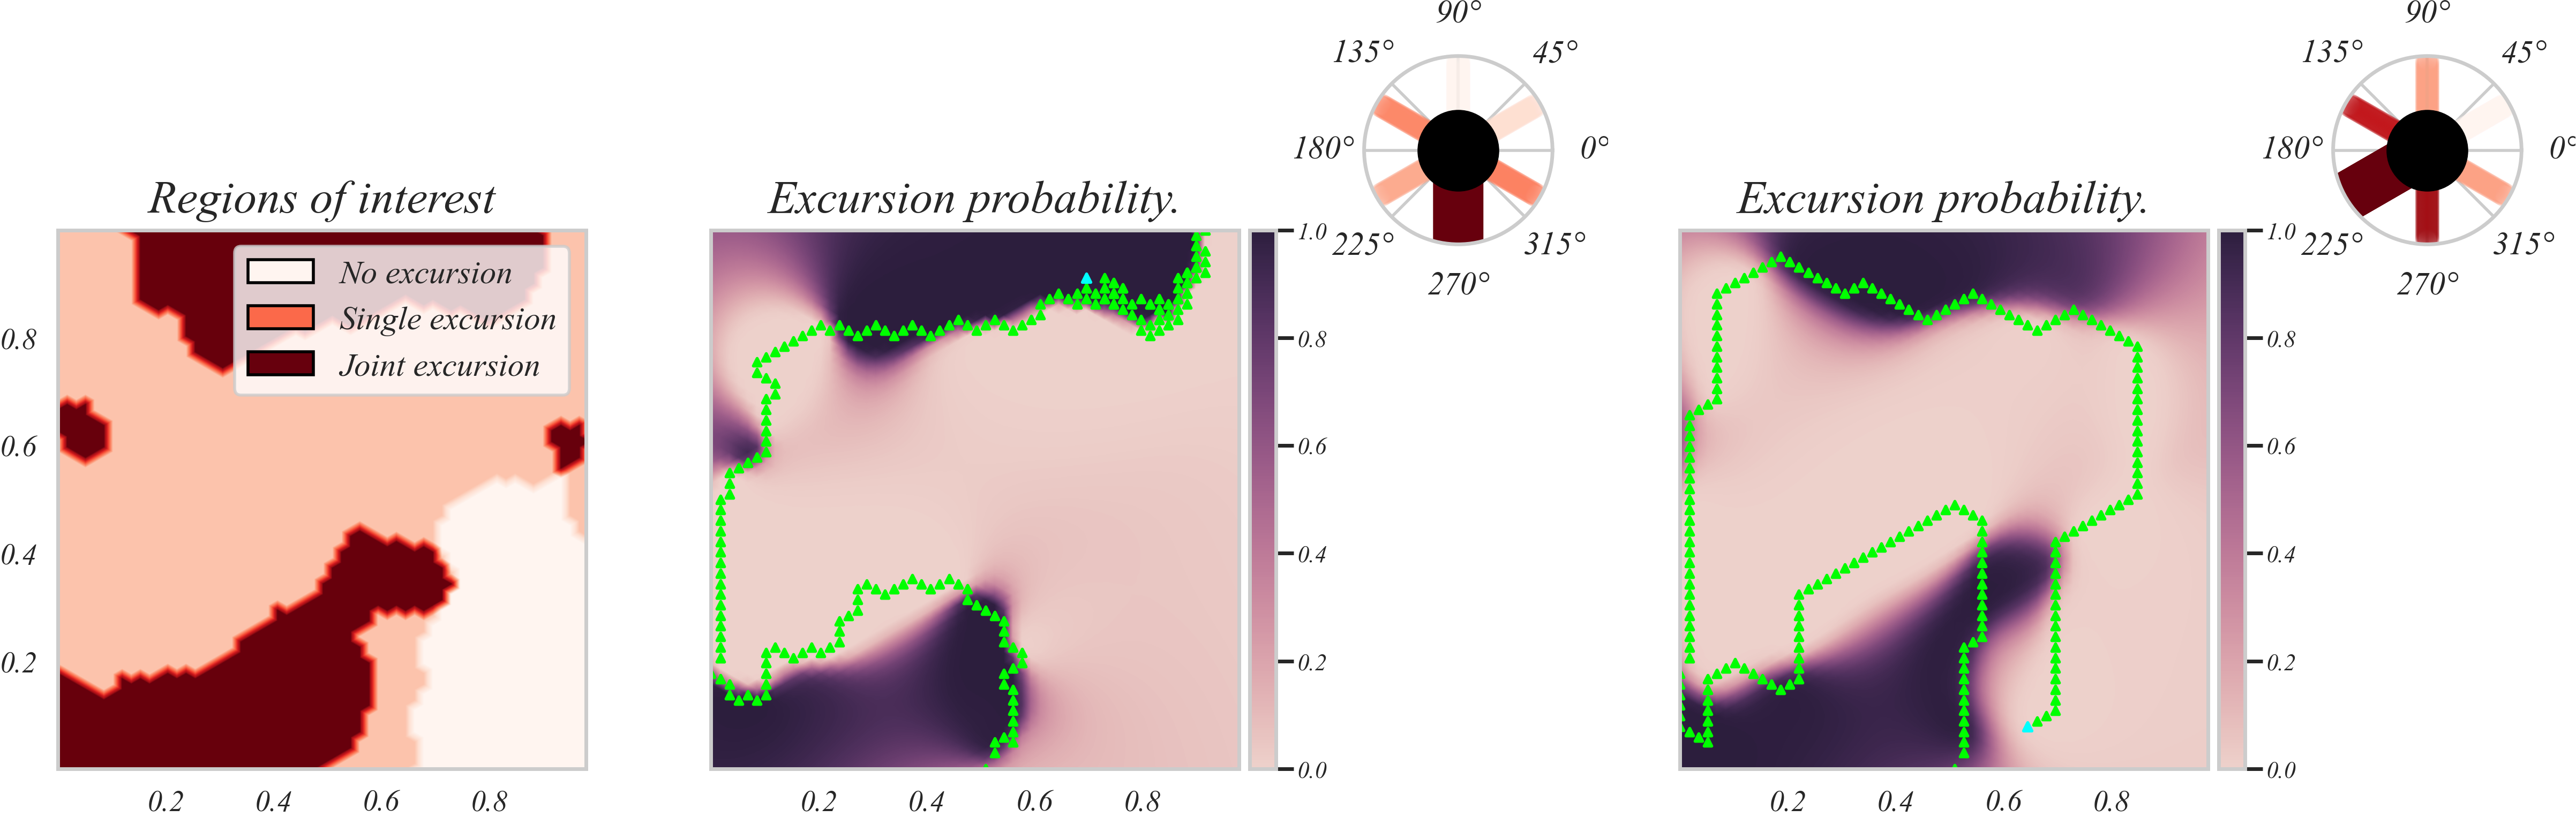
\includegraphics[scale=0.41]{ans_to_reviewers/merged_paths_2.png}
    \caption{Comparison of sampling paths and posterior EPs for different values of the measurement noise standard deviation (from left to right: $0.1$ and $0.5$). The sampling has been stopped after 200 steps.}
    \label{fig:nugget_comparison}
\end{figure}


\footnotesize
\bibliographystyle{imsart-nameyear}
\bibliography{ref}

\end{document}